\section{Graph Parsing Algorithm}
We propose a context-free language constrained path problem solution which allows to find all paths in graph. Paths are satisfied specified arbitrary context-free grammar. The algorithm constructs implicit representation of result. The results are represented with parsing forest of all possible parsing trees. 
Finite representation of result set with structure related to specified grammar may be useful not only for results understanding and processing but also for query debugging especially for complex queries. 

Our solution is based on generalized LL (GLL)~\cite{scott2010gll, FastPracticalGLL} parsing algorithm which allows to process ambiguous context-free grammars.
%Complexity is $O(n^3)$ in worst case and linear for unambiguous grammars, that better than complexity of CYK and Earley which used as base in other solutions (for example~\cite{ConjCFPathQuery}, ~\cite{GraphQueryWithEarley}).
%This fact allow to demonstarte better performance on linear subgraphs and unambiguous grammars.
%Also it is not necessary to transform input grammar to CNF which required for CYK which allow to avoid grmmar size decreasing.
%It is important because real performance of parsing algorithm is sensetive to grammar size.


\subsection{Generalized LL Parsing Algorithm}

Generalized LL (GLL) is generalized top-down parsing algorithm which handle all context-free grammars (including left recursive) with worst-case cubic time complexity and linear for LL grammars.
GLL is native for grammar, can be simple created !!!!!!! and debugging. Generalised algorithms look through all possible derivation in grammar for input. If current parsing branch is wrong the analisys (!??) process cotinious with others. 
GLL uses descriptors mechanism to store all parsing branches. Descriptors are four (!!???!!) elements which fully (??!!!) describes current parser state. Descriptor is a quadriple $(L, s, j, a)$ where $L$ is a line label, $s$ is a stack node, $j$ is a position in the input, and $a$ is a node of derivation tree. GLL parsers, like recursive descent parsers, consist of functions for every nonterminal and one dispatching function. Every function has label and a function gets control from another function due the call by the name. Process of analisys consist of calling function and tarts from the function for start nonterminal. !!!!!!!!!!!!!!!  нужно перейти от того, что лэйблы в оригинале и у нас!!!!!!!!!
Stack in parsing process is used to store return information for the parser --- a name of function which would be called when current function will stop work. As previously mentioned, generalised parsers process all possible derivation branches. For every branch parser must store it's own stack. It leads to OOM. !!!!  
Graph structured stack (GSS)~\cite{Tomita} is used to solve this problem. GSS allows to combine stacks to prevent duplication. Stacks with common part are combined to one graph structure and it stores only one node for evey analysis branch except whole stack. It allows to reduce (требуюмую) memory significantly. 
In GLL each GSS node contains pair --- position in input and grammmar slot. Grammar slot is like LR-slot. Slot is a grammar rule and position in it (for example !!!!).

The next part of the descriptor is a tree node. Parsers build derivation tree using input and grammar. There are more than one tree for ambigious grammar and generalised algorithms builds all derivation trees. Special data structure -- SPPF -- is used to reduce space required for tree storage.


\begin{algorithm}[h]
\begin{algorithmic}[1]
\caption{Single vertex processing}
\label{processVertex}
\Function{dispatcher}{}
  \If{$R.Count \neq 0$}  
      \State{$(L,v,i,cN) \gets R.Get()$}
      \State{$cR \gets dummy$}
      \State{$dispatch \gets false$}
  \Else
      \State{$stop \gets true$}
  \EndIf
\EndFunction

\Function{processing}{}
  \State{$dispatch \gets true$}
  \Switch{$L$}
  \Case{$(X \rightarrow \alpha \cdot x \beta)$ where $x = input[i + 1])$}
       \If{$cN = dummyAST$} 
          \State{$cN \gets \Call{getNodeT}{i}$} 
       \Else 
          \State{$cR \gets \Call{getNodeT}{i}$}
       \EndIf
       \State{$i \gets i + 1$}
       \State{$L \gets (X \rightarrow \alpha x \cdot \beta)$}
       \If{$cR \neq dummy$}
          \State{$cN \gets \Call{getNodeP}{L, cN, cR}$} 
       \EndIf
       \State{$dispatch \gets false$}        
  \EndCase
  \Case{$(X \rightarrow \alpha \cdot x \beta)$ where $x$ is nonterminal}
       \State{$v \gets$ \Call{create}{$(X \rightarrow \alpha x \cdot \beta), v, i, cN$}}
       \State{$slots \gets pTable[x][input[i]]$}
       \ForAll{$L \in slots$}
          \State{\Call{add}{L,v,i,dummy}} 
       \EndFor
  \EndCase
  \Case{$(X \rightarrow \alpha \cdot )$}
       \State{\Call{pop}{v,i,cN}} 
  \EndCase
  \Case{$\_$}
       \State{final result processing and error notification} 
  \EndCase
  \EndSwitch
\EndFunction

\Function{control}{}
  \While{not $stop$}  
      \If{$dispatch$}
        \State{\Call{dispatcher}{}}
      \Else
         \State{\Call{processing}{}}
      \EndIf
  \EndWhile
\EndFunction

\end{algorithmic}
\end{algorithm}

\subsection{Shared packed parse forest}

Shared Packed Parse Forest (SPPF)~\cite{SPPF} is a spetial data structure for derivation forest compact representation which allow to reuse common nodes and subtrees.
As a result multiple derivation trees, which can be produced in case of ambiguos grammar, can be compressed in one SPPF with optimal reusing of common parts.  
Binarized form of SPPF proposed in~\cite{brnglr} and it allow to achive worst-case cubic space complexity.
GLL can use SPPF~\cite{gllParsingTree} for results representation achive cubic space complexity with binarised version.

Let we present an example of SPPF for ambiguos grammar $G_0$ (pic~\ref{grammarG0}).

\begin{figure}[h]
   \begin{center}
\begin{verbatim}
   0: s = NUM
   1: s = L s R
   2: s = s s
\end{verbatim}
   \caption{Grammar $G_0$}
   \label{grammarG0}        
   \end{center}
\end{figure}

Here \verb|N| is token for number, \verb|L| and \verb|R| are tokens for '(' and ')'  respectively.

Let we parse the sentence \verb|"()()()"|. 
There are two diferent lefmost derivations of this sentence in grammar $G_0$ ($\rightarrow ^ n$ denote an application of production with nimber $n$): 
\begin{enumerate} 
    \item $s \rightarrow ^ 2 s s \rightarrow ^ 2 s s s \rightarrow ^ 1 L s R s s \rightarrow ^ 0 L N R s s \rightarrow ^ 1 
    L N R L s R s \rightarrow ^ 1 L N R L s R s \rightarrow ^ 0 L N R L N R s \rightarrow ^ 1 L N R L N R L s R \rightarrow ^ 0 L N R L N R L N R$
    \item $s \rightarrow ^ 2 s s \rightarrow ^ 1 L s R s  \rightarrow ^ 0 L N R s \rightarrow ^ 2 L N R s s  \rightarrow ^ 1 
    L N R L s R s \rightarrow ^ 1 L N R L s R s \rightarrow ^ 0 L N R L N R s \rightarrow ^ 1 L N R L N R L s R \rightarrow ^ 0 L N R L N R L N R$
\end{enumerate}
 
    As far as there are tho different derivations, SPPF should contains two different trees and it is presented in figure~\ref{sppfSample}: result SPPF(fig. ~\ref{sppf}) and trees for derivation 1(fig.~\ref{tree1}) and derivation 2(fig.~\ref{tree2}) respectively. 
 
\begin{figure*}[ht]
    \begin{center}
    \centering
    \begin{subfigure}[b]{0.3\textwidth}
        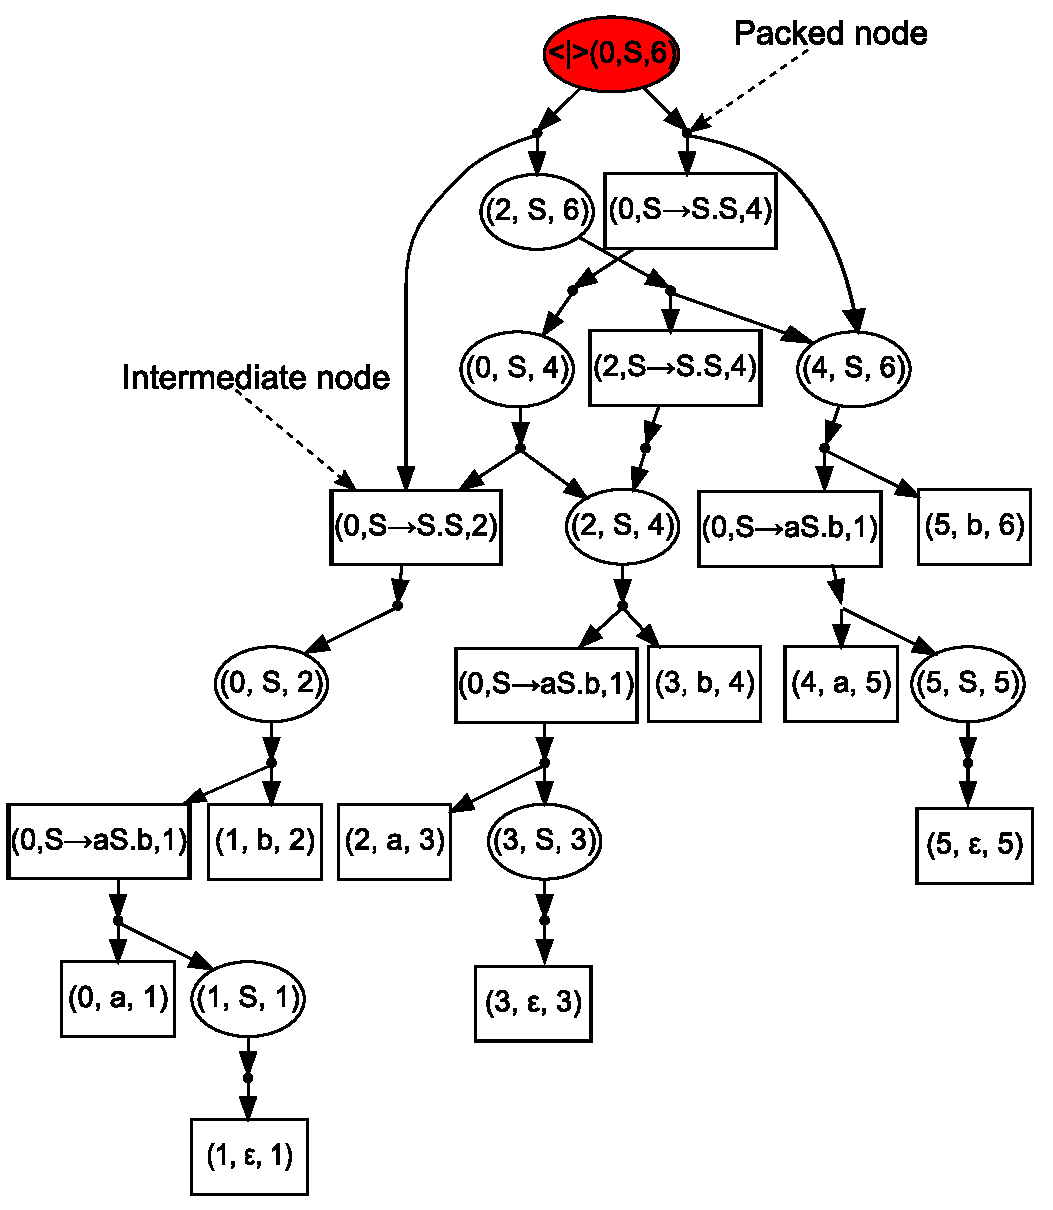
\includegraphics[width=\textwidth]{dot/Brackets.pdf}
        \caption{SPPF}
        \label{sppf}        
    \end{subfigure}
    ~
    \begin{subfigure}[b]{0.3\textwidth}
        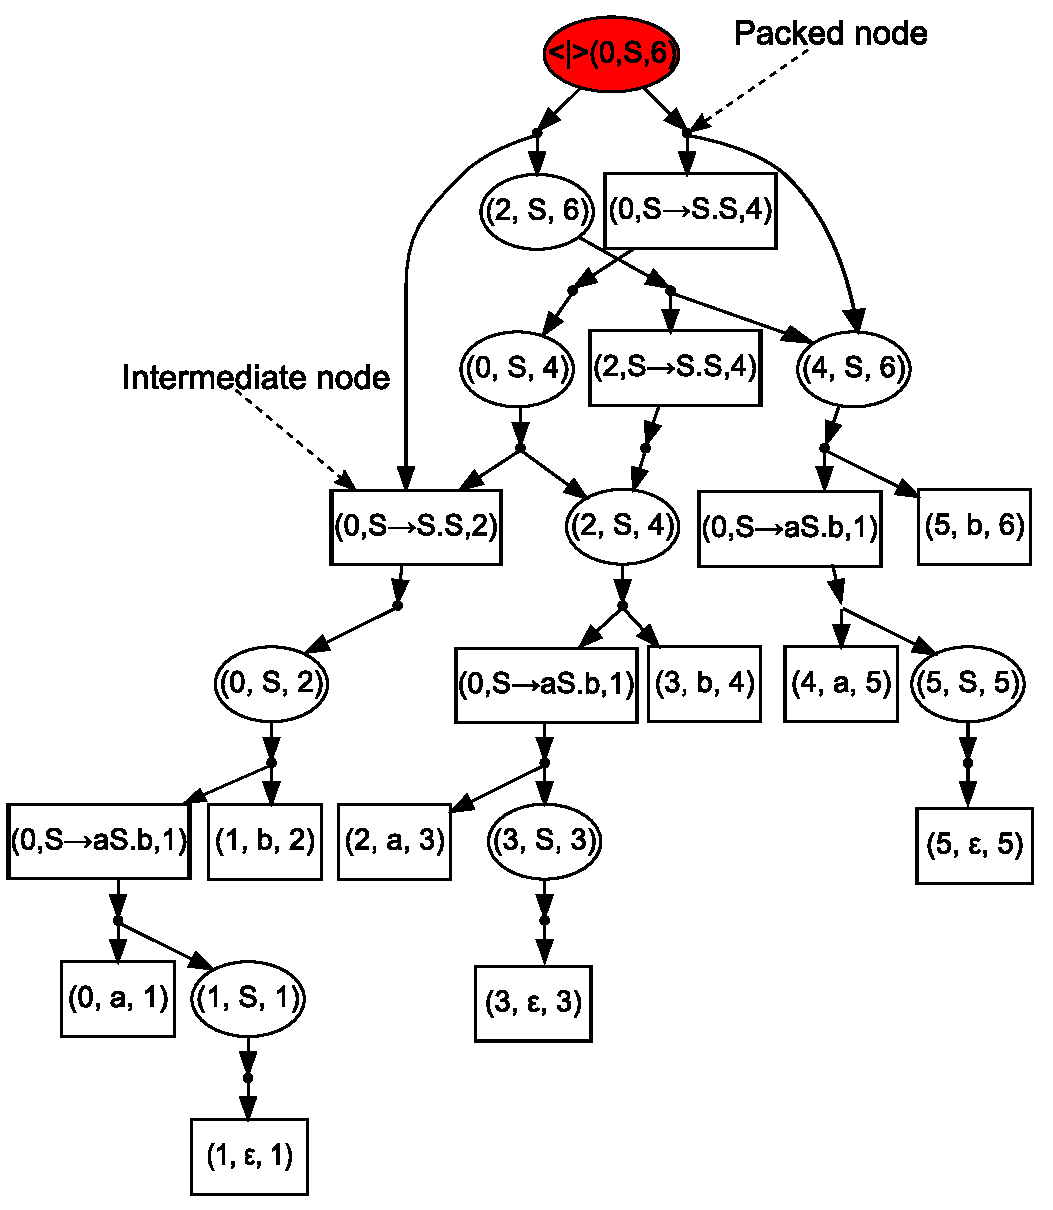
\includegraphics[width=\textwidth]{dot/Brackets.pdf}
        \caption{Tree for derivation 1}
        \label{tree1}        
    \end{subfigure}
    ~
    \begin{subfigure}[b]{0.3\textwidth}
        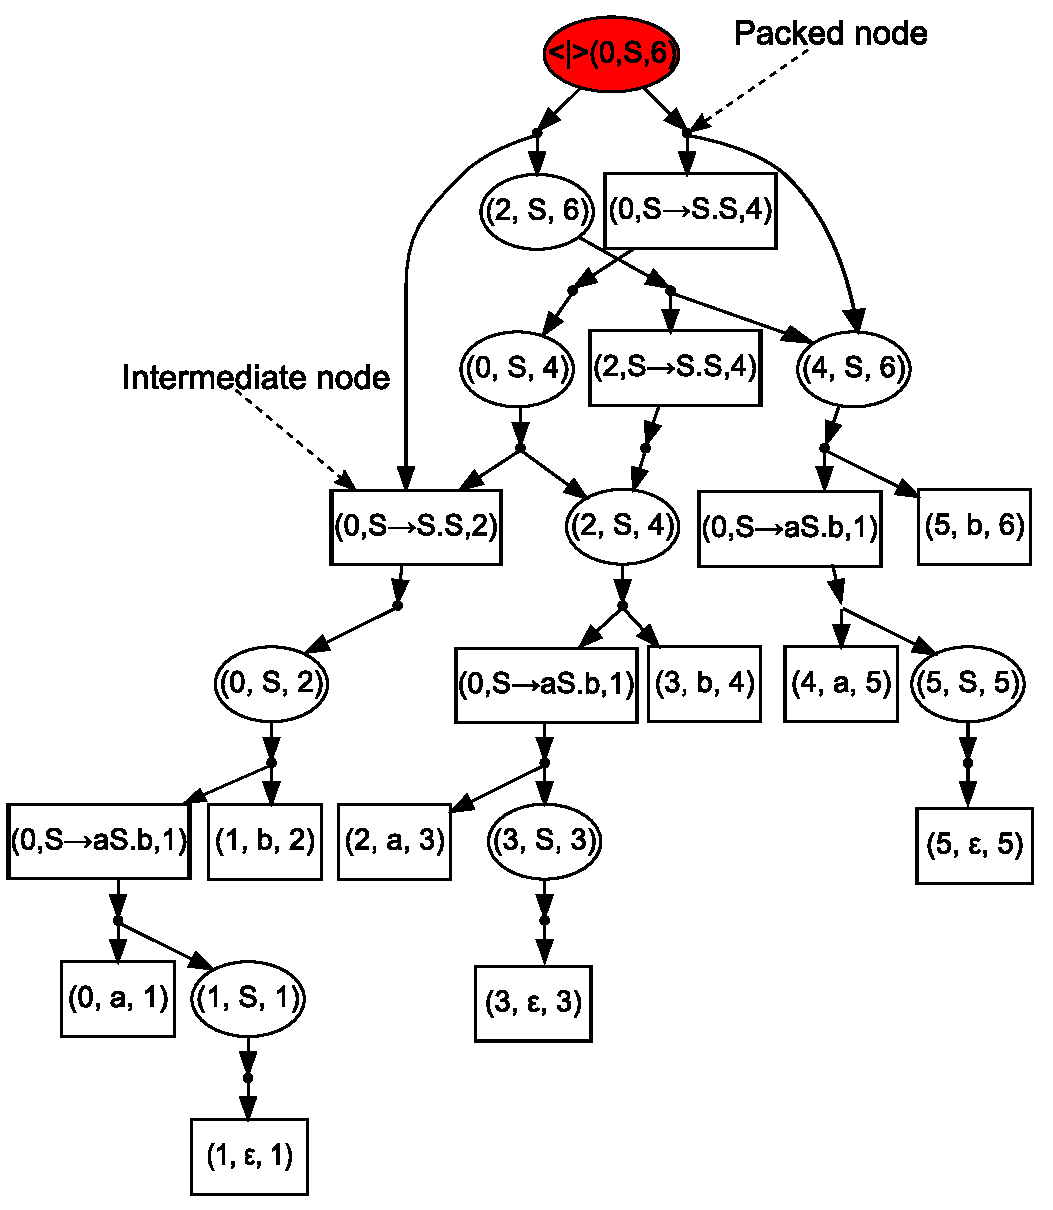
\includegraphics[width=\textwidth]{dot/Brackets.pdf}
        \caption{Tree for derivation 2}
        \label{tree2}        
    \end{subfigure}
    \caption{SPPF for sentence \textbf{\texttt{"(1)(2)(3)"}} and grammar $G_0$}
    \label{sppfSample}
    \end{center}                
\end{figure*}

Binarised SPPF can be represented as a graph where each node has one of four types: 

\begin{itemize}
    \item terminal node with label $(i,T,j)$;
    \item nonterminal node with label $(i,N,j)$;
    \item intermidiate node with label $(t,i,j)$ where $t$ is a grammar slot;
    \item packed node with label $(N : \gamma \cdot, k)$;
\end{itemize}
, and one of nodes can be marked as 'root' --- node for start nonterminal.

Further in our examples we will remove redudant intermidiate and packed nodes from SPPF to simplify it and decrease size of structure.

\subsection{GLL-based graph parsing}
(!!!!!Нужен какой-то переход или рассказ про то, как мы в виде графа представляем вход!!!!!!11)
In order to adapt GLL for graph parsing we need only use graph verticea as position in input.
As far as we work with context-free languages it is not important how this descriptor was created, and so descriptors management and other basic mechanisms of original algorithm can be reused ``as is''. 
We can merge it if they are equal. (!!!!!!!ВОТ эти два предожения вообще не нужны, кажется, но надо подумать!!!!!!!!!!!!!!) 

We implement some optimizations:~\cite{FastPracticalGLL}

We also use binarised SPPF for result representation whish allow to simplify query debugging and result explortion. (!!!!!!А что это  зачем?!!!!!!!)
In our case more then one root may be specified. For example, look at picture!!!! 
We 

$\mathbb{P}:G, M, StartVset, FinalVSet \rightarrow SPPF$
In details, main function input is graph $M$, set of start vertices $V_s\subseteq V$, set of final vertices $V_f\subseteq V$, grammar $G_1$.
Output is Shared Packed Parse Forest (SPPF)~\cite{SPPF} --- finite data structure which contains all derivation trees for all paths in $M$, $\Omega(p) \in L(G_1)$ and allows to reconstruct any of paths implicitly.
As far as we can specify sets of start and final vertices, our solution can find all paths in graph, all paths from specified vertex, all paths between specified vertices. 
Also SPPF represents a structure of paths in terms of derivation which allow to get more useful 
information about result. 
Binarized SPPF is at most cubic in terms of result size. 
Any path can be extracted in the linear time.

A bit more on corectnes.!!!!!
